\documentclass{article}
\usepackage{tikz, comment}
\usepackage{pifont}
\usepackage{fontspec, pgfplots}
\usetikzlibrary{arrows, decorations.markings, decorations.pathreplacing}
\begin{comment}
:Title: Not defined yet
:Tags: absolute value rules;parabola;cardioid;inverse of a matrix, matrix inverse , multiplicative inverse of a matrix ;absolute value of a complex number, modulus of a complex number 
:Prob: 0.5066;0.4608;0.4517;0.4426;0.4336
:Author: Prof.Hu Ji-shan, HKUST
:Slug: No name yet

Description Here.........
\end{comment}
\begin{document}\centering 

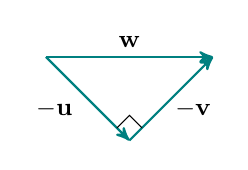
\begin{tikzpicture}[>=latex,xscale=.5*3, yscale=.5*3][font=\sf\small] 

\draw[teal, thick, ->, >=stealth'] ({-1/sqrt(2)}, {1/sqrt(2)}) --(0,0) node[black, left, midway, pos=0.5, xshift=-2, yshift=-4, scale=1]{$-\bf u$}; %-u

\draw[teal, thick, ->, >=stealth'] (0, 0) -- ({1/sqrt(2)}, {1/sqrt(2)})node[black, right, midway, pos=0.5, xshift=-2, yshift=-4, scale=1]{$-\bf v$}; %-v

\draw[teal, thick, ->, >=stealth'] ({-1/sqrt(2)}, {1/sqrt(2)})--({1/sqrt(2)}, {1/sqrt(2)})node[black, above, midway, pos=0.5, xshift=0, yshift=0, scale=1]{$\bf w$}; %w

\draw ({0.15*cos(pi/4 r)}, {0.15*sin(pi/4 r)}) -- (0, {0.15*sqrt(2)}) -- ({0.15*cos((3*pi/4) r)}, {0.15*sin((3*pi/4) r)});

\end{tikzpicture}
\end{document}